% -----
% COMP2300 cheat sheet for final exam
% Jimmy Lin
% -----
% -
\documentclass[8pt,a4paper,landscape]{article}
% package used
\usepackage{setspace}
%{{{
\usepackage{geometry,amsthm,amsmath,graphicx}
\usepackage[colorlinks,
            linkcolor=blue,
            anchorcolor=red,
            citecolor=green
            ]{hyperref}
\usepackage{verbatimbox}
\usepackage{tikz,multicol,amsfonts,wallpaper}
\geometry{top=1mm,bottom=1mm,left=2mm,right=2mm}
%}}}
% file info macros and package parameters
%}}}
% new command definition
\newcommand{\topic}[1]{\textbf{\large #1}}
\newcommand{\nl}{\vspace*{5mm}}
\newcommand{\hs}{\hspace*{3mm}}
% - 
\begin{document}
% title page
\small
\begin{spacing}{-1}
\begin{multicols*}{3}
    \noindent
    \topic{Quick look up} \\
    Hexadecimal: Aa-10  Bb-11  Cc-12  Dd-13  Ee-14  Ff-15 \\
    4 bits – nibble, 8bits – Byte, 2 Bytes – Word, 4 Bytes - Double Word\\
    KiB MiB GiB TiB PiB $2^{10n} Bytes = 1024^{n} Bytes$\\
    KB MB GB TB PB  $1000^{n} Bytes$ \\
    \hrule \noindent
    \topic{Linux command} \\
    \textbf{ltrace}: lists the library calls made by a running process as it is running. 
    \textbf{strace}: list the system calls.  \\
    \textbf{touch}: change timestamp / create an empty file. \\
    \textbf{cat}, \textbf{sort}, \textbf{uniq}, \textbf{echo} \\
    \textbf{stat}: information of a file. \textbf{file}: brief information of a file.\\
    \textbf{od}: show content of file in various ways. -c character -d \\
    \textbf{dd}: copy part of file. dd if=.. bs=BUFFER count=NBYTES of=.. \\
    \textbf{cp}: copy a whole file. \textbf{head}: filter first few lines of content. \\
    \topic{Special Files} \\
    \textbf{/dev/null}: black hole. \textbf{/dev/zero}: all zeros. \\
    \textbf{/dev/random}: full of random number. \\
    \textbf{/dev/mem}: overview of main memory. \\
    \textbf{/dev/hda}: raw block of hard disk. \\
    \hrule \noindent
    %% rPeANUt look up
\vspace*{-2mm}
\topic{rPeAnut} \\
\begin{verbatim}
xvar : block #1 ; a global variable xvar initialized to 1
xvar: block 10 ; an array xvar of length 10, all values 0
str: block #''abcde'' ; apply for a string
load #xvar R0 ; load address of xvar to R0 (immediate load)
load xvar R0 ; load the value in xvar to R0 (absolute load)
store R3 xvar ; value in address R3 to xvar (indirect rest)
store R3 #xvar R0; global variable as base 
store R0 #-1 SP ; store for return value in recursion
p1.x = 4 differ to pp1 -> x = 4 in what you load from
p1.x load from #p1 , p1 -> x load from pp1  \end{verbatim}
    \textbf{negate}:flip all bits then plus 1. \textbf{not}: just filp all bits \\
    \textbf{rotate}:most significant bit will turn back to the least bit \\
    status 0xFFF1, IO control 0xFFF2 represents? \\
\hrule \noindent
\topic{File operation}
\begin{verbatim}
/* scanf, fscanf, malloc, free */
scanf("%10s", p);
fscanf(fp,"%[^,]%*%lf\n", people[i].n, &people[i].h) != EOF 
int* p = (int *) malloc ( sizeof(int) * 100 );
free(p);

/* open, read, write */ 
int open(const char * pathname, int flags, mode_t mode)
// returns a 'file descriptor', a small non-negative 
//   number which provides a reference to the opened file.

int  read(  int  handle,  void  *buffer,  int  nbyte ); 
// returns 0 at the end of file

int  write(  int  handle,  void  *buffer,  int  nbyte  );
// The function returns the number of bytes written to file.
// A return value of -1 indicates an error.

// lseek: move current file offset 
off_t lseek(int fd, off_t offset, int whence);
----------------------------------------------------------
/* File open example */
#include <stdio.h> 
int main() { 
    FILE *pFileS = fopen( "s.rar", "rb" );
    if(!pFileS ) return 1; 
    FILE *pFileD = fopen( "d.rar", "wb" ); 
    unsigned char buffer[ 4 * 1024 ];
    int nRead;
    while(nRead = fread( buffer, sizeof(unsigned char),
            sizeof(buffer), pFileS) ) 
        fwrite(buffer, sizeof(unsigned char), nRead, pFileD); 
    fclose( pFileS ); fclose( pFileD );
    return 0;
}
\end{verbatim}
\hrule \noindent
\topic{Network operation} \\
\textbf{inet\_ntop()} . \\
A string containing an IP address in readable form, and you want to pack it into a struct sockaddr\_in or a struct sockaddr\_in6. In that case, the opposite funcion inet\_pton() \\
inet\_ntop() returns the dst parameter on success, or NULL on failure (and errno is set). \\
inet\_pton()returns1on success. It returns-1if there was an error (errno is set), or 0 if the input isn't a valid IP address. \\

\begin{verbatim}
// inet_add return a long integer
ina.sin_addr.s_addr = inet_addr("132.241.5.10");
/* reverse conversion by inet_ntoa */
a1 = inet_ntoa(ina1.sin_addr); // result is 198.92.129.1 
printf("address 1: %s ",a1);	// address 1: 132.241.5.10
---------------------------------------------------------
// IPv4 demo of inet_ntop() and inet_pton()
struct sockaddr_in sa;
char str[INET_ADDRSTRLEN];
// store this IP address in sa:
inet_pton(AF_INET, "192.0.2.33", &(sa.sin_addr));
// now get it back and print it
inet_ntop(AF_INET, &(sa.sin_addr), str, INET_ADDRSTRLEN);
printf("%s\n", str); // prints "192.0.2.33"
---------------------------------------------------------
// IPv4 demo of inet_ntop() and inet_pton()
struct sockaddr_in sa;
char str[INET_ADDRSTRLEN];
// store this IP address in sa:
inet_pton(AF_INET, "192.0.2.33", &(sa.sin_addr));
// now get it back and print it
inet_ntop(AF_INET, &(sa.sin_addr), str, INET_ADDRSTRLEN);
printf("%s\n", str); // prints "192.0.2.33"
\end{verbatim}

\vspace*{-3mm}
    \hrule \noindent
    \topic{Basics} \\
    \textbf{FLOP}: floating point operation per second. \\
    \textbf{Mbps}: Mega bit per second. \textbf{MIPS}: Mega instruction persecond. \\
    \textbf{Endianness}: the order the bytes within a single word are stored within main memory. 
    \textbf{Big endianness} -- most significant byte first. \\  
    Way to represent negative number: \\
    1. simple offset: normal addtion does not work. \\ 
    2. reserve 1-bit as sign bit: range -127 to 127. \\
    3. 2s complement: take advantage of 1 and 2.  \\
    \textbf{2s complement}: range -127 to 128 \\
    negate value: flip all bits and plus 1. \\
    overflow flag: result is too large to be represented. \\
    \textbf{Fixed point}: $(-1)^s m b^e$  \\
    \textbf{IEEE 754 floating point}:  1 sign bit, 8 exp bits, 23 significand \\
    subnormal: $(-1)^s \times 0.m \times 2^{e-126}$. 
    normal: $(-1)^s \times 1.m \times 2^{e-127}$. \\
    \textbf{Special case}: exp $0xFF$, if $m = 0$, value = inf. else, value = NaN \\

    \hrule \noindent
    %% concepts of first few chapters
    \topic{Introduction}  \\
    \textbf{Abstraction}: with multiple levels of detail / description, it helps manage complexity and provides interfaces and standards. \\
    \textbf{Virtualization}: gives the appearance of a capability or service. This decouples the service from the underlying physical resources. It helps in terms of simplicity, flexibility and resource sharing. \\
    \textbf{Prototypes}: signatures of functions will be used in code. \\
    \textbf{Static keyword} reduces the scope to the file it is within.\\
    \hrule \noindent
    \topic{Files and File System} \\
    \textbf{system call}: is how a program requests a service from an operating system's kernel. \\
    In Linuxe Based x86 machines, system calls are performed by generating interruption, 
    which is trapped by kernel and then processed. \\
    A \textbf{FILE} is a named collection of related information.  \\
    A \textbf{file system} provides a uniform logical view of related information. \\
    Two ways to READ/WRITE files: \\
    \hs \textbf{system calls}: open, read, write, ioctl.\\
    \hs \textbf{file streams}: fopen, fread, fwrite. \\
    \textbf{mmap}:file can be mapped into memory, done by the 'mmap' function. 
    \textbf{mmap} enables the file's contents to be view and modified in normal memory. \\
    \textbf{SHARED mmap}: modifications to the memory of the mapped file are written back to the actual file, also other processes that maps the same file sees the same modifications. \\
    \textbf{PRIVATE mmap}: process has its own private copy of the file. Modifications are not written back to the file and other processes do not see any changes. \\
    \textbf{Fixed File Descriptor (int fd)}: stdin - 0,stdout - 1, stderr - 2 \\
    res = read(0,buf,255);   res = write(1,"Hello",6); \\
    \textbf{3 access files methods}:sequential/direct/memory mapped access

    \hrule \noindent
    \topic{Structure of C program} \\
    Source  $\rightarrow$  (COMPILE) $\rightarrow$   assemble code(.s) $\rightarrow$   
    (ASSEMBLE) $\rightarrow$  object code(.o) $\rightarrow$  (LINK) $\rightarrow$  executable \\
    \textbf{malloc} returns a pointer to the amount of memory requested.(free)
    \textbf{struct} may add padding to make certain types are appropriately aligned in memory.
    
    \hrule \noindent
    \topic{Interrupts} \\
    \textbf{Interrupt}, \textit{an event alters the normal fetch-decode-execution}. When occurred, current program will be suspended. caused by hardware event and software event. \\
    Interrupt handler should be carefully designed such that the state of CPU returns exactly how it was found. \\
    \textbf{Interrupt latency}: time between an interrupt occur and code executed to handle it. \\
    \textbf{Interrupt storm}: Interrupts occur more frequently than the handler can serve, then requests to handle interrupts will be lost.

    \hrule \noindent
    \topic{Memory} \\
    \textbf{Dynamic random access memory (DRAM)} only requires \textit{a single transistor and capacitor per bit}, this enables much higher density memory (compared with SRAM). However, it is considerably slower and more complex to access. \\
    \textbf{Static random access memory (SRAM)} is fast volatile memory that is simple to interface with. SRAM will be found in: CPU caches, buffers for various devices within a computer system. \\
    \textbf{ROM} is non-volatile so state is maintained without power. \\
    \textbf{Flash memory} is an electronic non-volatile computer storage device that can be electrically erased and reprogrammed. \\
Registers, L1 cache, L2 cache, DRAM, Flash Drive, Magnetic Disk Drive, Network Backup Server. 
    (\textit{capacity increase, speed decrease}.)

\hrule \noindent
2 basic approaches for the design of the control unit. \\
\textbf{Hardwire}: these control units basically are finite state machines that are specially designed to sequence the CPU based on the instruction it is executing. (not particularly flexible and can be difficult to design, however, good performance) \\
\textbf{Microcode}: this approach uses ROM type memory within the CPU to act like machine code for sequencing the different action within the CPU. simpler and more flexible approach. \\

\hrule \noindent
\topic{CPU performance} \\
CPUs have moved caches onto the CPU die which enables the CPU to be physically closer to the cache. This \textbf{reduces latency}. \\
\textbf{Pipeling}: involves in lots of independent stages, IF, ID, E, WB. \\
\textbf{Superscale} architectures involve duplicate functional units within the cpu and then start one instruction on the same clock cycle in the pipeline. Enables larger throughput of instructions. \\
Sometimes instructions will require data from memory before they can execute, this will stall the pipeline. \textbf{Slow the CPU}. \\
\textbf{Outer of order execution} approach loads the next few instructions and starts executing the instruction that has the required data. \\
\textbf{Multithread}: CPUs can maintain the programming context of multiple threads (so \textit{duplication of state and register information}), without the duplication of processing units, caches, TLBs, etc, This enables multiple threads to be executed within the one core and hide latency. 
\textbf{Multicores}: The CPU can be duplicated, share the same memory and L2 Cache.

\hrule \noindent
\topic{CPU Cache} \\
\textbf{Cache hit}: occur when data required by instruction is in cache. \\
\textbf{Cache miss}: occur when data required is \textit{not} in cache.\\
\textbf{Write-through}: written to cache and main memory at same time. \\
\textbf{Write-back}: data is just written to cache. \\

\hrule \noindent
\topic{Linking} \\
\textbf{Binding of instructions and data} to memory addresses may occur at: compile time, load time, or execution time. \\
\textbf{Linking for libraries}:
\textbf{statically linked}: the library is compiled into the final binary executable.
\textbf{dynamically linked}: just a 'stub' is includes in the binary executable, 
the library code is obtained as needed during execution.

\hrule \noindent
\topic{Processes} \\
\textbf{A context switch} changes the process a CPU is executing. \\
A \textbf{thread} is the basic unit of execution within a process. \\
Lightweight process (LWP, traditional, has only one thread). \\
Each thread, consists of a program counter, a register set and a stack space. \\
A \textbf{process} consists of a group of threads. They share text, data, opened files, capabilities, etc. \\
\textbf{CPU-cache}(SRAM) stores copies of main memory data.. \\
\textbf{Working set} is the memory that a program is currently using
fully associative cache, direct mapping cache, set associative cache. \\

\hrule \noindent
\topic{Memory Management and Paging} \\
\textit{Addresses generated by the CPU} are called \textbf{logical addresses}. 
These are the addresses 'seen' by the user's programs.\\
\textit{Addresses seen by the main memory} are called \textbf{physical addresses}. \\
\textbf{Physical memory} is divided into \textit{fixed-sized blocks called frames}. \\
\textbf{Logical memory} is div into \textit{blocks of the same size called pages}. \\
Logical addresses (produced by the CPU) are divided into \textit{two parts: the page number and the offset}. 
\textbf{Each process has a page table}. \\
\textbf{Memory Management Unit}: responsible for mapping from logical address to physical address. \\
\textbf{Page table}: responsible for logical address to physical address. If it is large, page table could be
stored in the main memory. \\
\textbf{Page Table Base Register (PTBR)}: points to the page table. A fast lookup cache may store the page frame mappings within CPU. \\
\textbf{Translation Look-aside Buffer (TLB)}: entry is the frame number. \\
\textbf{Internal Fragmentation}: the whole frame occupation by process causes waste. \\
\textbf{Segmentation}: A user or process would like to view memory as a set of variable-sized segments. Each segment has a name and there is no necessary ordering among segments. \\
\textbf{Advantages of separating logical \& physical addresses}: \\
1.execution-time address binding.  4.simplifies sharing of data. \\
2.simplifies the swapping of processes in and out of memory. \\
3.protection / security of data between processes.
\hrule \noindent
\topic{Virtual Memory} \\
\textbf{Swapping} is an approach that involves bringing an entire process from disk into main memory so it may be executed. \\
\textbf{Demand-paging} is a lazy "swapper" which brings into memory the pages of the process that are needed. \\
One approach to paging is to only bring pages into memory when they are needed. This is called Pure demand paging. \\
\textbf{Advantages of paging}:
1. programs can be larger than physical memory \\
2. abstracts main memory into an extremely large logical storage area \\
3. increases the degree of multi-programming \\
swap space generally is faster than the file system (as file lookups and indirect allocation methods are not used) \\
\textbf{page replacement methods}: \\
1. frame-allocation algorithm \\
2. page-replacement algorithm(FIFO, OPT/MIN, LRU, LFU)\\
valid-invalid bit: hardware support \\
\hrule \noindent
\topic{CPU Scheduling} \\
In \textbf{multiprogramming systems}, the running task keeps running until it performs an operation that requires waiting for an external event (e.g. reading from a tape) or until the computer's scheduler forcibly swaps the running task out of the CPU. (multiprogramming is a CPU scheduling strategy.) \\
There are two \textbf{types of schedulers}: \\
1. non-preemptive - CPU is not 'forcefully' taken from the process. \\
2. preemptive - CPU may be forcefully taken from the process and switched to another process. \\
\textbf{Criteria of scheduling algorithms}: \\
1. CPU utilization - percentage of time the CPU is in use. \\
2. Throughput - rate at which processes are being completed. \\
3. Turnaround time - interval of time from the starting a process to completing the process. \\
4. Wait time - amount of time a process spends in the ready queue. \\
5. Response time - The amount of time it takes a process to start responding. This does not include the time to output the
response. \\
\textbf{Three algorithms for CPU Scheduling}: \\ 
1. First Come First Serve (FCFS) \\
2. Shortest Job First (SJF) provably shortest waiting time \\
3. Round Robin (RR): each time CPU excution no more than a threshold. \\

\hrule \noindent
%% Networks
Most \textbf{Ethernet controllers} have unique 48bit MAC address. \\
\textbf{Ethernet's topology} started as \textit{bus} topology. But now LAN would generally use \textit{star} topology with a switch at the center. \\
\textbf{Weakness of bus topology}: Only one device may transmit information to the bus at any time. If two units transmit at the same time a collision will occur, both transmission with usually be compromised and will need to be re-transmitted.

\hrule \noindent
%% UDP/TCP
\textbf{Particular IP Address}: \\
0.0.0.0 - This host (only source), 127.X.X.X - loopback.
\\
10.X.X.X - private network, 192.168.X.X - private network. \\
255.255.255.255 - Broadcast on the local network. \\
\textbf{IPv4} (Internet Protocol) provides \textit{32bit addresses (decimal)} for addressing computing devices that span the globe. \\
\textbf{TCP} (Transmission Control Protocol) provides a way of sending larger amounts of data to particular 'ports' on a host.
and resend missing packets and check that packets arrive in the correct order. \\
\textbf{UDP} (User Datagram Protocol): unreliable way, without a connection to be setup, not order check but very fast. \\


\hrule \noindent
%% 1-bit register flip flop diagram
\textbf{1-bit register component diagram}
\begin{center}
    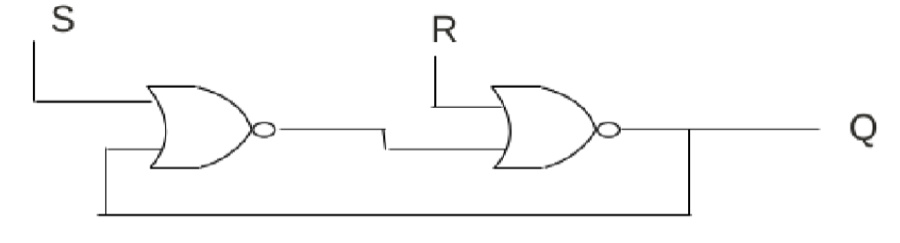
\includegraphics[width=2in,height=1in]{./flip-flop.png} \\
\end{center}

\end{multicols*}
\end{spacing}
\end{document}
